\section{Training}
\begin{frame}{}
    \LARGE GANs: \textbf{Training}
\end{frame}

\begin{frame}[allowframebreaks]{Training}
\begin{itemize}
    \item Both Discriminator and Generator are trained jointly in a min-max game.
    \item Minimax objective function:
    $$\min_{\theta_G} \max_{\theta_D} = E_{x \sim p_{data}} log(\underbrace{D_{\theta_D}(x)}_{\substack{\text{Discriminator}\\ \text{output for}\\ \text{real data }x}}) + E_{x \sim p(z)} log(1-\underbrace{D_{\theta_D}(G_{\theta_G}(z))}_{\substack{\text{Discriminator output}\\ \text{for generated fake}\\ \text{data } G(z)}})$$
    \item Discriminator $\theta_D$ wants to maximise objective such that $D(x)$ is close to 1 (real) and $D(G(z))$ is close to 0 (fake).
    \item Generator $\theta_G$ wants to minimise objective such that $D(G(z))$ is close to 1 (discriminator is fooled into thinking generated $G(z)$ is real).

\end{itemize}

\framebreak
\begin{figure}
    \centering
    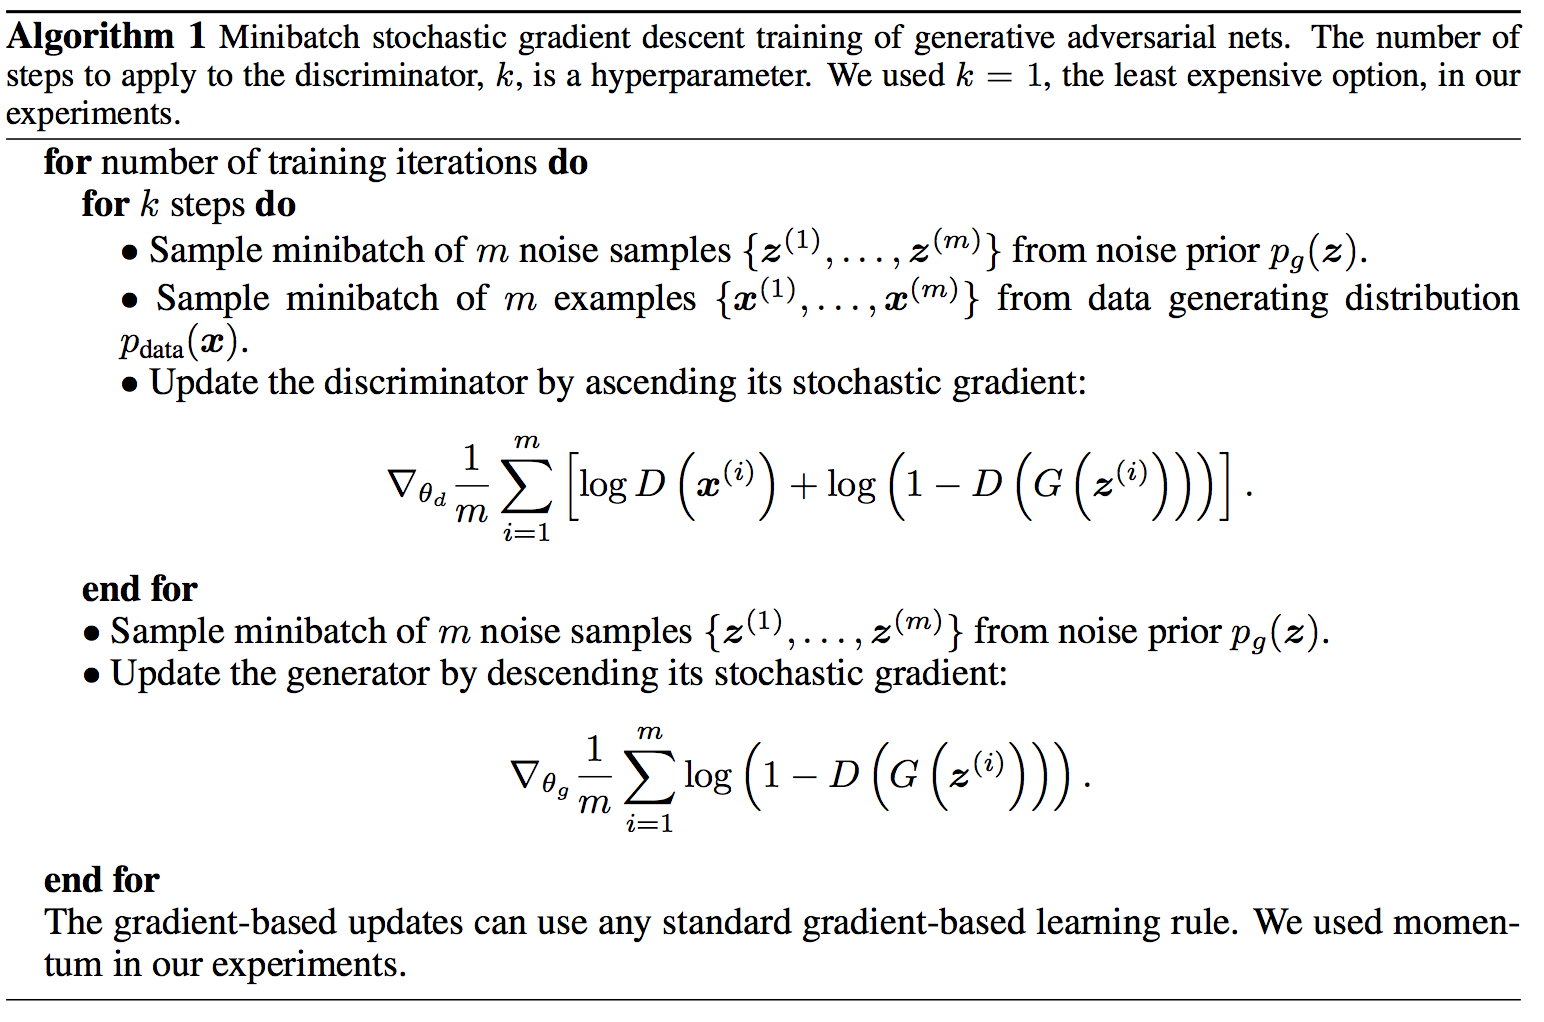
\includegraphics[height=1\textheight, width=1.02\textwidth, keepaspectratio]{images/gan/pseudocode.png}
\end{figure}

\framebreak
\textbf{The Adversarial Process:}
\begin{enumerate}
    \item Discriminator is trained to distinguish real from fake.
    \item Generator is trained to fool the discriminator.
    \item Repeat: Alternate steps until convergence.
\end{enumerate}

\textbf{Training Tips:}
\begin{itemize}
    \item Use batch normalization.
    \item Avoid sigmoid output in discriminator.
    \item Use Leaky ReLU in discriminator.
\end{itemize}

\textbf{Practical Issues:}
\begin{itemize}
    \item Discriminator becomes too strong.
    \item Gradient vanishing for generator.
    \item Careful balance of training speeds is necessary.
\end{itemize}
    
\end{frame}